%\documentclass[a4paper,10pt,hungarian]{report}
%\documentclass[a4paper,10pt,hungarian]{article}
\documentclass[a4paper,10pt]{article}
%a ,,hungarian'' opci� csak a draftcopy csomaghoz kell!
%\usepackage[latin2]{inputenc}
%\usepackage[T1]{fontenc}
%\usepackage[magyar]{babel}
\usepackage[left=2.5cm,right=2.5cm,top=2cm,bottom=2cm]{geometry}
\usepackage{indentfirst}
\usepackage{upgreek}
\usepackage{relsize}
\usepackage{hyperref}
\usepackage{ifthen}
\usepackage{scrextend}
\addtokomafont{labelinglabel}{\sffamily}
\usepackage{tikz}
\usetikzlibrary{calc,fit,arrows,positioning}
\sloppy
%\usepackage{graphicx}
%\usepackage{ifthen}
%\usepackage{multicol}
%\usepackage[outline]{draftcopy} %outline,bottom,light,none/first/firsttwo
%\usepacgake{wasysym}
%%%% Don't modify next two line! %%%%
%.PDF.\usepackage{times}
%.PDF.\usepackage[T1]{mathtime}
\frenchspacing
\newcommand{\mypi}{{\larger $\uppi$}}
%\newcommand{\mypi}{{\larger $\pi$}}
\newcommand{\pifs}{\mypi{}fs}
\newcommand{\pifsl}{Pi file system}
\newcommand{\fname}[1]{\texttt{#1}}
\newcommand{\code}[1]{\texttt{#1}}

%%% TiKZ
\tikzstyle{block} = [draw,fill=yellow!20,dashed,minimum size=2.5cm,inner sep=0.45cm]
\tikzstyle{blocktext} = [text width=2.4cm,align=left]
\tikzstyle{page} = [draw,fill=brown!25,dashed,minimum width=2cm,minimum height=0.8cm,text width=1.6cm,align=left]
\tikzstyle{flash} = [draw,fill=gray!15,inner sep=0.45cm]
% diameter of semicircle used to indicate that two lines are not connected
\def\radius{.7mm} 
\tikzstyle{branch}=[fill,shape=circle,minimum size=3pt,inner sep=0pt]
\makeatletter
\tikzset{
    dot diameter/.store in=\dot@diameter,
    dot diameter=2pt,
    dot spacing/.store in=\dot@spacing,
    dot spacing=8pt,
    dots/.style={
        line width=\dot@diameter,
        line cap=round,
        dash pattern=on 0pt off \dot@spacing
    }
}
\makeatother
% Define layers, otherwise gray blocks will hide pages
\pgfdeclarelayer{background}
\pgfdeclarelayer{background2}
\pgfsetlayers{background,background2,main}
%%% End of TiKZ

\author{Peter Ivanov \textless{}ivanovp@gmail.com\textgreater{}}
\title{\pifsl{} (\pifs{})}
%%
%\usepackage[dvips]{graphicx}

%%

\begin{document}
\maketitle
%\tableofcontents
\section{Introduction}
This file system was developed for embedded systems which use NOR flash as 
storage. 
The development started as teach-myself project and I released the code in 
hope that it will be useful for someone else as well. 

NOR flash ICs have very low price nowadays (2017) and can be used
to store files. But there are few problems to consider when designing a file
system:
\begin{itemize}
\item NOR flashes can be programmed (set bits to zero) by pages, but only 
can be erased (set bits to one) in a larger quantity, which are mostly called
block in the datasheets. One page is usually 256 or 512 bytes, one block 
consits of 16, 256, 1024, etc. pages. So typical block sizes are 4 KiB, 
64 KiB, 256 KiB.
\item Blocks can be erased ~10,000--100,000 times. After that data retention is 
not guaranteed. Therefore all blocks should be erased uniformly. This method 
is called wear leveling.
\end{itemize}

\pifs{} can be scaled from 4 Mbit (512 KiB), 256 Mbit (32 MiB), 
theoretically up to 1 Gbit (128 MiB) memory sizes.

The code is not MISRA compatible, but I've written MISRA code earlier and I 
tend to use the rules.
So I tried to use 'return' only at the end of functions, use 'break'
once in 'while' cycles or not use it at all and call one function from 
expressions (or not call functions at all from expressions). I didn't use
'goto' in the sources of file system, but you may find them in STM32 HAL's 
sources.

\subsection{Features of the \pifs{}}
\begin{itemize}
\item Small memory footprint
\item Files can be opened for update ("r+", "w+", "a+" modes are supported)
\item Size of logical page is user-defined
\item Cache buffer for page (currently only one page is cached)
\item Directory handling
\item Dynamic wear-leveling
\item Static wear-leveling (limited, work-in-progress)
\item User data can be added for files: permissions, owner IDs, etc.
\item At the beginning of flash memory reserved blocks can be defined, which 
are not used by the file system
\end{itemize}

\subsection{Limitations of the \pifs{}}
\begin{itemize}
\item Only one flash chip can be used (one volume is supported)
\item Memory and file system configuration cannot be changed during run-time
\item One directory can only store pre-defined number of files or directories
\item No OS support yet, file system can be used only from one task
\item Incompatible with FAT file system, therefore cannot be used for USB mass
storage devices
\end{itemize}

\section{Definitions, Acronyms and Abbreviations}
\begin{labeling}{File system header} % <--- here goes the longest definition to measure the necessary space
\item[NOR flash] Special type of EEPROMs, which manufactured using NOR gates.

\item[Page] Array of several bytes in the flash memory. Number of bytes is 
power of two, usually 256 or 512 bytes. See \autoref{fig:flash}.

\item[Block] Composed of several pages. Usually a block contain 16, 256 or 1024
pages. See \autoref{fig:flash}.

\item[Logical page] Allocation unit of file system. User configurable option.
Larger logical page needs more RAM and less pages in management area.
Smaller logical page needs less RAM and more pages in management area.
It shall be larger or equal to page size. 
Define: \code{PIFS\_LOGICAL\_PAGE\_SIZE\_BYTE}

\item[Erase] Change data bits to one (logical high level). Only a whole block 
can be erased, which means all bits of the block are set to one.

\item[Program] Change data bits to zero (logical low level). Each bit of a page
can be programmed individually.

\item[Block address] Index of block in flash memory. 
Type: \code{pifs\_block\_address\_t}

\item[Page address] Index of a page in a block. It can be flash page address
for flash functions or logical page address for file system's functions.
Type: \code{pifs\_page\_address\_t}

\item[Page offset] Index of a byte in a page. It can be flash page offset
for flash functions or logical page offset for file system's functions.
Type: \code{pifs\_page\_offset\_t}

\item[Data area] Blocks which hold the file's content. 
See \autoref{fig:flashfs}.

\item[Management area] Blocks which hold the file system's internal
data, how much space is allocated, where are the data pages of files, etc. There are two types of management area: primary (active) management area, secondary (next) management area.
See \autoref{fig:flashfs}.

\item[File system header] First page of active management area contains the
header of file system. It describes address of free space bitmap, entry list,
delta map, wear level list, etc.
Type: \code{pifs\_header\_t}, variable: \code{pifs.header}.

\item[FSBM] Free space bitmap. It stores information about all logical pages 
of flash memory:
1 bit stores whether page is free, 1 bit stores if page is to be released.

\item[Delta page] If content of a file is overwritten and original page
cannot be overwritten because bits should be changed from 0 to 1, delta pages 
are added. When the original page is read from a given address the content of
delta page is provided from a different address.

\item[Map page] Management page which is used to describe data pages of a file.

\item[Entry list] Technically a directory of file system. If directories are
disabled, only root entry list exist.

\item[Entry] One file or directory in the directory.

\item[TBR] To be released. A page which was used, but now it can erased then 
allocated. If all pages in a block marked TBR, the block can be erased.

\item[Merge] During merge management area is written, blocks are erased, delta pages are resolved and entry list is compacted. The data is copied from primary to secondary management area and the next secondary management area is selected.
\end{labeling}

\begin{figure}[ht]
\centering
%%%%%%%%%%%%%%%%%%%%
%%% Flash figure %%%
%%%%%%%%%%%%%%%%%%%%

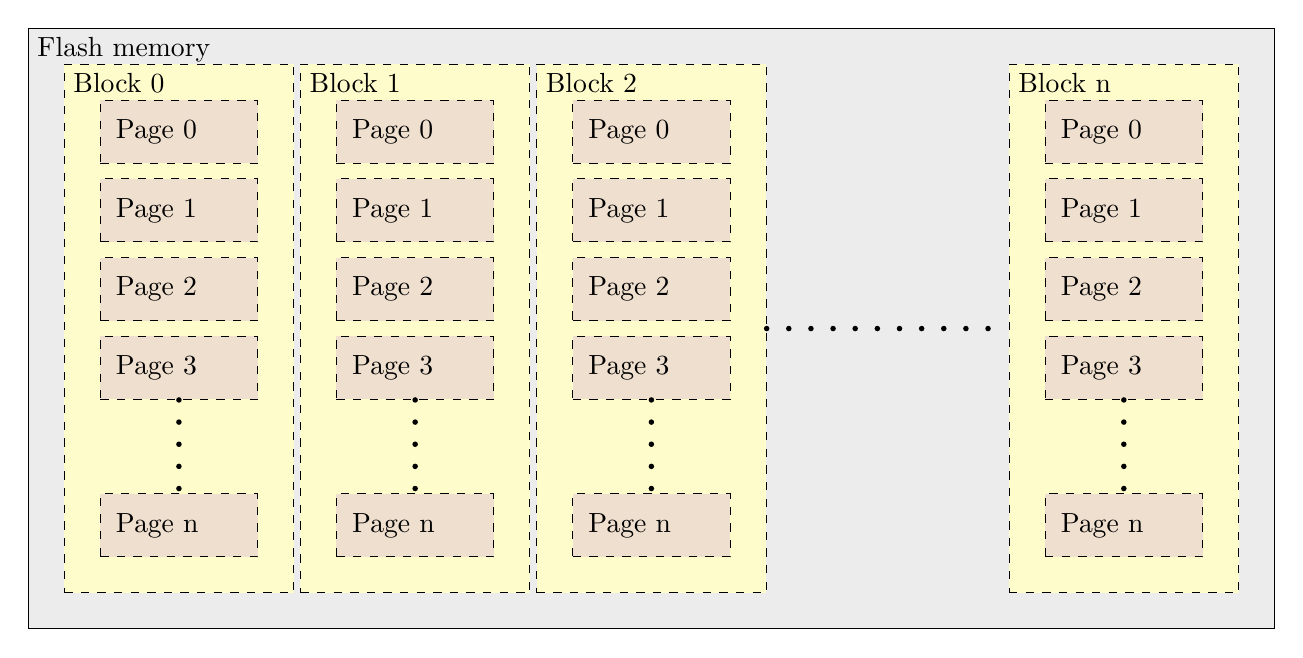
\begin{tikzpicture}[>=latex']
%%% Draw blocks 0..2
\foreach \x in {0,1,2} {
    % Draw pages
    \foreach \y in {0,1,2,3} {
        \node[page] at (\x * 3,-\y) (page\x\y) {Page \y};
    }
    \def\y{5}
    \node[page] at (\x * 3,-\y) (page\x\y) {Page n};
    \draw[dots] (page\x3) -- (page\x\y);
    \begin{pgfonlayer}{background2}
    % Draw block
    \node[fit=(page\x0) (page\x\y), block] (block\x){};
    \node[below right,blocktext] at (block\x.north west) {Block \x};
    \end{pgfonlayer}
}
%%% Draw block n
\def\x{4}
% Draw pages
\foreach \y in {0,1,2,3} {
    \node[page] at (\x * 3,-\y) (page\x\y) {Page \y};
}
\def\y{5}
\node[page] at (\x * 3,-\y) (page\x\y) {Page n};
\draw[dots] (page\x3) -- (page\x\y);
\begin{pgfonlayer}{background2}
% Draw block
\node[fit=(page\x0) (page\x\y), block] (block\x){};
\draw[dots] (block2) -- (block\x);
\node[below right,blocktext] at (block\x.north west) {Block n};
\end{pgfonlayer}

\begin{pgfonlayer}{background}
\node[fit=(block0) (block4),flash] (flash){};
\node[below right] at (flash.north west) {Flash memory};
\end{pgfonlayer}
\end{tikzpicture}

\caption{Flash memory layout}
\label{fig:flash}
\end{figure}

\begin{figure}[ht]
\centering
%%%%%%%%%%%%%%%%%%%%%%%
%%% Flash FS figure %%%
%%%%%%%%%%%%%%%%%%%%%%%

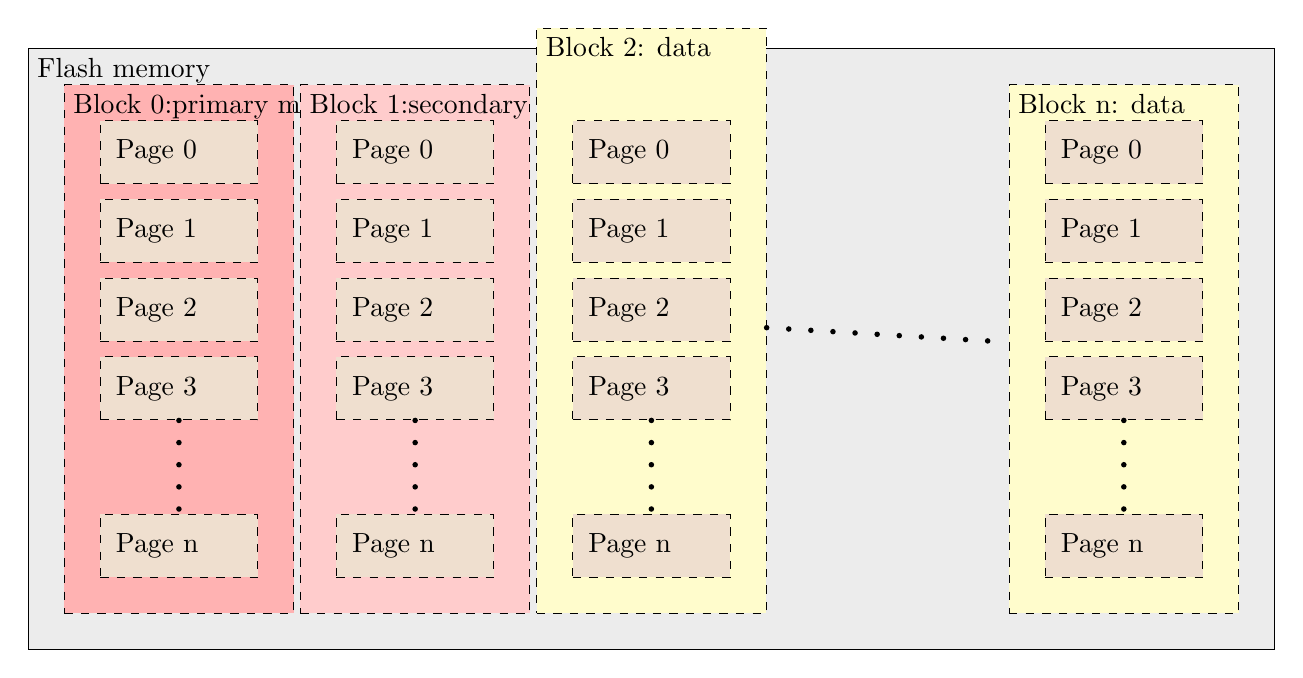
\begin{tikzpicture}[>=latex']
%%% Draw blocks 0..2
\foreach \x in {0,1,2} {
    % Draw pages
    \foreach \y in {-1,0,1,2,3} {
        \ifthenelse{-1 = \y}
        {
            % Invisible!
            \node[draw=none] at (\x * 3,-\y) (page\x\y) {};
        }
        {
            \node[page] at (\x * 3,-\y) (page\x\y) {Page \y};
        }
    }
    \def\y{5}
    \node[page] at (\x * 3,-\y) (page\x\y) {Page n};
    \draw[dots] (page\x3) -- (page\x\y);
    \begin{pgfonlayer}{background2}
    % Draw block
    \ifthenelse{0 = \x \OR 1 = \x}
    {
        \ifthenelse{0 = \x}
        {
            % primary management
            \node[fit=(page\x0) (page\x\y), block,fill=red!30] (block\x){};
            \node[below right] at (block\x.north west) {\hbox{Block \x: \newline
            primary management}};
        }
        {
            % secondary management
            \node[fit=(page\x0) (page\x\y), block,fill=red!20] (block\x){};
            \node[below right] at (block\x.north west) {\hbox{Block \x: \newline
            secondary management}};
        }
    }
    {
        % data
        \node[fit=(page\x-1) (page\x\y), block] (block\x){};
        \node[below right] at (block\x.north west) {Block \x: data};
    }

    \end{pgfonlayer}
}
%%% Draw block n
\def\x{4}
% Draw pages
\foreach \y in {-1,0,1,2,3} {
    \ifthenelse{-1 = \y}
    {
        % Invisible!
        \node[draw=none] at (\x * 3,-\y) (page\x\y) {};
    }
    {
        \node[page] at (\x * 3,-\y) (page\x\y) {Page \y};
    }
}
\def\y{5}
\node[page] at (\x * 3,-\y) (page\x\y) {Page n};
\draw[dots] (page\x3) -- (page\x\y);
\begin{pgfonlayer}{background2}
% Draw block
\node[fit=(page\x0) (page\x\y), block] (block\x){};
\draw[dots] (block2) -- (block\x);
\node[below right] at (block\x.north west) {Block n: data};
\end{pgfonlayer}

\begin{pgfonlayer}{background}
\node[fit=(block0) (block4),flash] (flash){};
\node[below right] at (flash.north west) {Flash memory};
\end{pgfonlayer}
\end{tikzpicture}
            
%\footnotetext{Primary management block}
%\footnotetext{Secondary management block}


\caption{Flash memory layout when \pifs{} installed}
\label{fig:flashfs}
\end{figure}

\section{Demonstration}
In the 'demo' directory three applications can be found.
\begin{enumerate}
\item pc\_emu: PC application which uses NOR flash emulator. It can be compiled
with GNU make an GCC.
\item maple\_mini\_pifs: Demo running on Maple Mini board, MCU is 
STM32F103RCBT6. There is no NOR flash, UART and debugger on board. So 
prototype should be created.
\item nucleo-f413zh\_pifs: Demo running on Nucleo-F413ZH board, MCU is
STM32F413ZH. There is no NOR flash memory on the board, some prototype hardware 
should be created.
It has internal debugger and virtual serial port. 
It can be compiled with GNU make and GCC or with STM32 System Workbench.
\item stm32\_f4ve\_pifs: Demo running on STM32-F4VE board, MCU is STM32F407VE. 
There is Winbond W25Q16DV NOR flash soldered on the board, but it has not got 
UART. 
So external debugger and USB-serial converter is needed.
It can be compiled with GNU make and GCC or with STM32 System Workbench.
\end{enumerate}

\subsection{Using demo}
All applications based on a command interpreter which communicates over UART.
There are commands to list directory, create and dump files, run some tests.

The commands:

\begin{labeling}{append} % <--- here goes the longest definition to measure the necessary space
\item[ls] List directory. Switches: \code{-l} display file size, \code{-e} 
examine file (for debugging). \code{-e} switch displays address of first
map page of file or entry list of directory.
\item[l] List directory with switches: -l and -e (for debugging).
\item[rm] Remove file. Switch: -a remove all files in the directory.
\item[dumpf] Dump file in hexadecimal format.
\item[df] Alias to \code{dumpf}.
\item[cat] Read and print file to console.
\item[create] Create file. You can type file until 'q' is entered in the 
first character of a line.
\item[append] Append to file. You can type file until 'q' is entered in the 
first character of a line.
\item[cd] Change directory. Only available if directories are enabled.
\item[mkdir] Make directory. Only available if directories are enabled.
\item[rmdir] Remove an empty directory. Only available if directories are 
enabled.
\item[cwd] Get current working directory. Only available if directories are 
enabled.
\item[dump] Read and show a flash page in hexadecimal format. First parameter
is the address, second optional parameter in number of flash pages to display.
Note: this command works with flash page size other ones work with logical 
page size!
Example: \code{dump 0x10000 2}
\item[d] Alias to \code{dump}.
\item[map] Decode and display a map page.
\end{labeling}

Example use of commands on a flash M25P40, where logical and flash page size 
are the same (256 bytes):
\begin{verbatim}
> l
List directory '.'
small0.tst                             512  BA1/PA13 @0x10D00
small1.tst                             512  BA1/PA14 @0x10E00
small2.tst                             512  BA1/PA15 @0x10F00
small3.tst                             512  BA1/PA16 @0x11000
small4.tst                             512  BA1/PA17 @0x11100
small5.tst                             512  BA1/PA18 @0x11200
> m 0x10D00
Map page BA1/PA13 @0x10D00

Previous map: BA255/PA65535 @0x1FEFF00
Next map:     BA255/PA65535 @0x1FEFF00

BA2/PA0 @0x20000  page count: 2
> d 0x20000 2
Dump page BA2/PA0 @0x20000
00020000 46 69 6C 65 3A 20 73 6D 61 6C 6C 30 2E 74 73 74   File: small0.tst
00020010 2C 20 73 65 71 75 65 6E 63 65 3A 20 30 23 00 00   , sequence: 0#..
00020020 10 00 11 00 12 00 13 00 14 00 15 00 16 00 17 00   ................
00020030 18 00 19 00 1A 00 1B 00 1C 00 1D 00 1E 00 1F 00   ................
00020040 20 00 21 00 22 00 23 00 24 00 25 00 26 00 27 00    .!.".#.$.%.&.'.
00020050 28 00 29 00 2A 00 2B 00 2C 00 2D 00 2E 00 2F 00   (.).*.+.,.-.../.
00020060 30 00 31 00 32 00 33 00 34 00 35 00 36 00 37 00   0.1.2.3.4.5.6.7.
00020070 38 00 39 00 3A 00 3B 00 3C 00 3D 00 3E 00 3F 00   8.9.:.;.<.=.>.?.
00020080 40 00 41 00 42 00 43 00 44 00 45 00 46 00 47 00   @.A.B.C.D.E.F.G.
00020090 48 00 49 00 4A 00 4B 00 4C 00 4D 00 4E 00 4F 00   H.I.J.K.L.M.N.O.
000200A0 50 00 51 00 52 00 53 00 54 00 55 00 56 00 57 00   P.Q.R.S.T.U.V.W.
000200B0 58 00 59 00 5A 00 5B 00 5C 00 5D 00 5E 00 5F 00   X.Y.Z.[.\.].^._.
000200C0 60 00 61 00 62 00 63 00 64 00 65 00 66 00 67 00   `.a.b.c.d.e.f.g.
000200D0 68 00 69 00 6A 00 6B 00 6C 00 6D 00 6E 00 6F 00   h.i.j.k.l.m.n.o.
000200E0 70 00 71 00 72 00 73 00 74 00 75 00 76 00 77 00   p.q.r.s.t.u.v.w.
000200F0 78 00 79 00 7A 00 7B 00 7C 00 7D 00 7E 00 7F 00   x.y.z.{.|.}.~..

Dump page BA2/PA1 @0x20100
00020100 80 00 81 00 82 00 83 00 84 00 85 00 86 00 87 00   ................
00020110 88 00 89 00 8A 00 8B 00 8C 00 8D 00 8E 00 8F 00   ................
00020120 90 00 91 00 92 00 93 00 94 00 95 00 96 00 97 00   ................
00020130 98 00 99 00 9A 00 9B 00 9C 00 9D 00 9E 00 9F 00   ................
00020140 A0 00 A1 00 A2 00 A3 00 A4 00 A5 00 A6 00 A7 00   ................
00020150 A8 00 A9 00 AA 00 AB 00 AC 00 AD 00 AE 00 AF 00   ................
00020160 B0 00 B1 00 B2 00 B3 00 B4 00 B5 00 B6 00 B7 00   ................
00020170 B8 00 B9 00 BA 00 BB 00 BC 00 BD 00 BE 00 BF 00   ................
00020180 C0 00 C1 00 C2 00 C3 00 C4 00 C5 00 C6 00 C7 00   ................
00020190 C8 00 C9 00 CA 00 CB 00 CC 00 CD 00 CE 00 CF 00   ................
000201A0 D0 00 D1 00 D2 00 D3 00 D4 00 D5 00 D6 00 D7 00   ................
000201B0 D8 00 D9 00 DA 00 DB 00 DC 00 DD 00 DE 00 DF 00   ................
000201C0 E0 00 E1 00 E2 00 E3 00 E4 00 E5 00 E6 00 E7 00   ................
000201D0 E8 00 E9 00 EA 00 EB 00 EC 00 ED 00 EE 00 EF 00   ................
000201E0 F0 00 F1 00 F2 00 F3 00 F4 00 F5 00 F6 00 F7 00   ................
000201F0 F8 00 F9 00 FA 00 FB 00 FC 00 FD 00 FE 00 FF 00   ................
> df small0.tst
File size: 512 bytes
Dump file 'small0.tst'
00000000 46 69 6C 65 3A 20 73 6D 61 6C 6C 30 2E 74 73 74   File: small0.tst
00000010 2C 20 73 65 71 75 65 6E 63 65 3A 20 30 23 00 00   , sequence: 0#..
00000020 10 00 11 00 12 00 13 00 14 00 15 00 16 00 17 00   ................
00000030 18 00 19 00 1A 00 1B 00 1C 00 1D 00 1E 00 1F 00   ................
00000040 20 00 21 00 22 00 23 00 24 00 25 00 26 00 27 00    .!.".#.$.%.&.'.
00000050 28 00 29 00 2A 00 2B 00 2C 00 2D 00 2E 00 2F 00   (.).*.+.,.-.../.
00000060 30 00 31 00 32 00 33 00 34 00 35 00 36 00 37 00   0.1.2.3.4.5.6.7.
00000070 38 00 39 00 3A 00 3B 00 3C 00 3D 00 3E 00 3F 00   8.9.:.;.<.=.>.?.
00000080 40 00 41 00 42 00 43 00 44 00 45 00 46 00 47 00   @.A.B.C.D.E.F.G.
00000090 48 00 49 00 4A 00 4B 00 4C 00 4D 00 4E 00 4F 00   H.I.J.K.L.M.N.O.
000000A0 50 00 51 00 52 00 53 00 54 00 55 00 56 00 57 00   P.Q.R.S.T.U.V.W.
000000B0 58 00 59 00 5A 00 5B 00 5C 00 5D 00 5E 00 5F 00   X.Y.Z.[.\.].^._.
000000C0 60 00 61 00 62 00 63 00 64 00 65 00 66 00 67 00   `.a.b.c.d.e.f.g.
000000D0 68 00 69 00 6A 00 6B 00 6C 00 6D 00 6E 00 6F 00   h.i.j.k.l.m.n.o.
000000E0 70 00 71 00 72 00 73 00 74 00 75 00 76 00 77 00   p.q.r.s.t.u.v.w.
000000F0 78 00 79 00 7A 00 7B 00 7C 00 7D 00 7E 00 7F 00   x.y.z.{.|.}.~..

00000100 80 00 81 00 82 00 83 00 84 00 85 00 86 00 87 00   ................
00000110 88 00 89 00 8A 00 8B 00 8C 00 8D 00 8E 00 8F 00   ................
00000120 90 00 91 00 92 00 93 00 94 00 95 00 96 00 97 00   ................
00000130 98 00 99 00 9A 00 9B 00 9C 00 9D 00 9E 00 9F 00   ................
00000140 A0 00 A1 00 A2 00 A3 00 A4 00 A5 00 A6 00 A7 00   ................
00000150 A8 00 A9 00 AA 00 AB 00 AC 00 AD 00 AE 00 AF 00   ................
00000160 B0 00 B1 00 B2 00 B3 00 B4 00 B5 00 B6 00 B7 00   ................
00000170 B8 00 B9 00 BA 00 BB 00 BC 00 BD 00 BE 00 BF 00   ................
00000180 C0 00 C1 00 C2 00 C3 00 C4 00 C5 00 C6 00 C7 00   ................
00000190 C8 00 C9 00 CA 00 CB 00 CC 00 CD 00 CE 00 CF 00   ................
000001A0 D0 00 D1 00 D2 00 D3 00 D4 00 D5 00 D6 00 D7 00   ................
000001B0 D8 00 D9 00 DA 00 DB 00 DC 00 DD 00 DE 00 DF 00   ................
000001C0 E0 00 E1 00 E2 00 E3 00 E4 00 E5 00 E6 00 E7 00   ................
000001D0 E8 00 E9 00 EA 00 EB 00 EC 00 ED 00 EE 00 EF 00   ................
000001E0 F0 00 F1 00 F2 00 F3 00 F4 00 F5 00 F6 00 F7 00   ................
000001F0 F8 00 F9 00 FA 00 FB 00 FC 00 FD 00 FE 00 FF 00   ................

End position: 512 bytes

\end{verbatim}

\end{document}
